\documentclass{report}

\usepackage{amsmath}
\usepackage{hyperref}
\usepackage{graphicx}

\graphicspath{ {./figures/} }

\begin{document}

\title{Scale- and Translation-Invariant Unsupervised Learning of Hidden Causes Using Spiking Neurons with Top-Down Attention}
\author{Youssef Kashef}
\date{7. August 2013}
\maketitle
\tableofcontents

\chapter{Abstract}

Nessler et al. have demonstrated the ability of a spiking neuronal network governed by spike-timing-dependent-plasticity (STDP) and a stochastic winner-take-all (WTA) circuit to learn and predict causes from visual input. We aim to increase the computational power of the existing network through invariance to translation and scale. The visual system of the brain masters the recognition of objects wherever they appear in the visual scene and regardless of scale, orientation or even with partial occlusions. It achieves this through attention. Therefore, we turn to the pool of literature on modeling visual attention systems inspired from the brain. The architecture of the extended model is composed of the existing recognition module whose response modulates the attention module to be constructed in a top-down manner. This modulation will allow the attention module to alter the input window exposed for recognition. Attention is modeled as a network measuring for saliency in a scene by feature extraction with the use of hierarchies. The design and development of this extended model to achieve the required invariance using processes that approximate their biological counterparts is presented. Emphasis is put on making these approximations through computationally economic implementations. Evaluation of the model is based on its performance in a set of experiments as well as its computational efficiency. Experiments are constructed to scrutinize the behavior of the model, its ability to converge onto a sight within a scene that enables recognition. Artificial as well as natural images are used to further reveal the capabilities and limitations of our approach.

\chapter{Introduction}

elaborated abstract with references.......\cite{Nessler2010}

\chapter{Object Recognition with Spike-based Expectation Maximization}

\section{Spike-based Expectation Maximization}

Literature review of existing SEM model

Nessler et. al articulate a model of bayesian modules of how the brain analyzes sensory stimuli. The model demostrates the learning of hidden causes in visual stimuli emerging through correlations in a stochasitc soft winner-take-all (WTA) network of spiking neurons activated continuously in the presence of their preferred stimulus \cite{Nessler2010}. It utilizes spike-timing-dependent-plasticity (STDP) in WTA circuits as an approximation of Expectation Maximization \cite{Nessler2013}. This model forms the basis of the presented work.

More emphasis will be put on how the WTA circuit in the SEM model is constructed. This WTA circuit constitutres our main building block. It comprises of a feed-forward single layer spiking neural network. The input layer is made out of spiking nodes whose firing activity is governed  by a poisson process. External variables undergo a population coding that determine the modality of this poisson process. In the example offered by Nessler the external variables are intensity values, pixels, form a static visual stimulus, an image. The population coding polarizes the pixel intensity values into binary on-off states which directly determine the firing probability of the poisson process. A spiking neuron is assigned to encode each state of the population code generated for each pixel. In this case two spiking nodes per pixel. An On-node and an Off-node. The firing rate of these neurons is proportional to the state of the node in the population code.

\section{SEM for learning features}

\subsection{Extending SEM by learning orientations}

The current encoding of external variables accounts for the intensities of the spatial units (pixels) of the presented stimulus. The encoding of intensities is performed through a population coding by antognistic binary nodes per pixel that drive a poisson process \cite{Nessler2010}. Parallel to these intensity encoded nodes, we add a WTA circuit per pixel that determines the preferred orientation of this node relative to its spatial neighbors. This creates an orientation map of the presented stimulus. Whilst counter-intuitive with traditional learning models, SEM benefits from elaborating the dimensionality of WTA
s feature space as this increases its resolution for detecting correlations between an output node $z$ and input nodes $y$ on a linear scale. Since SEM aims to reduce dimensionality, it is preferable to describe it as an elaboration of dimensionality. The added dimensions, or nodes, do not carry new information, but rather refine its representation. Recalling the use of using population coding to encode in atagonistic (On-node, Off-node) fashion, thus letting the WTA learn the likelihood of an input node firing and not firing explicitly, as shown by \ref{eqn_corr}.

\begin{equation}
	p(z=1|y) \propto y*p(y=1|z) + (1-y)*p(y=0|z)
	\label{eqn_corr}
\end{equation}

where
\begin{itemize}
  \item $z$ denotes an output node,
  \item $y$ denotes an input node
\end{itemize}

As we introduce the orientation map we may add additional operands to \ref{eqn_corr} to account for the node's preferred orientation.

\begin{equation}
	\begin{split}
		p(z=1|y_I \cup y_O) \propto &y_I*p(y_I=1|z) + (1-y_I)*p(y_I=0|z) \\
			&+ y_o*p(y_O=O_p|z)+\sum_{i\neq o_i} (1-y_O)p(y_O=o_i|z)\\
	\end{split}
	\label{eqn_corr2}
\end{equation}

where
\begin{itemize}
  \item $y_I$ denotes an input intensity node,
  \item $y_O$ denotes an orientation input node,
  \item $O$ denotes the set of orientations available. Orientations can be defined discretly and arbitrarily (e.g. 30, 60,...180 degrees) or they can be learned \cite{Nessler2010},
  \item $O_p$ denotes the preferred orientation
\end{itemize}

We redesign the network with a cascade of hierarchical WTA circuits. The input layer is a matrix of WTA circuits per pixel. Each input WTA circuit decides on the preferred orientation and intensity of its input. We will experiment with configuring the input WTA circuit to only relay intensity, or only orientation, or both information.

The WTA circuits responsible to determine the preferred orientation of all input nodes are activated by convoling the stimulus with a bank of two-dimensional Gabor filters. The filters are defined with different scales and angular orientations from a predefined discrete set. By comparing the magnitude of responses between the filters at each pixel we can decide on the pixel's preferred orientation. Talking about the preferred orientation of a pixel would not actually make a lot of sense. The transfomations do yield responses for each pixel but they only becomes informative in relation to the responses of its neighbors.

\begin{figure}[h]
\centering
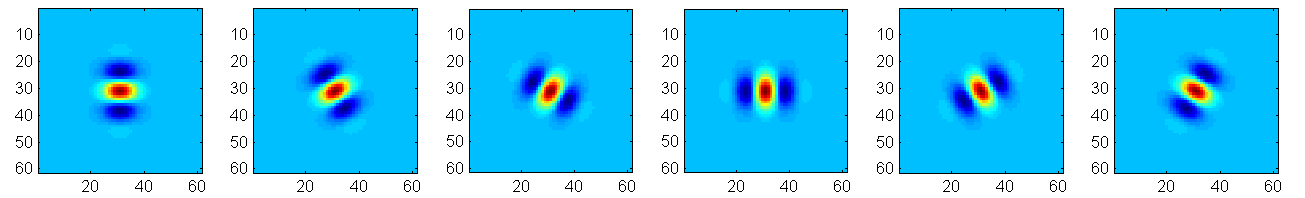
\includegraphics[width=0.8\textwidth]{filters_real}
\caption{Example of Gabor filters (real part). Defined at orientations [0, 150] degrees with 30 degrees increments. \label{fig:filters_real}}
\end{figure}

Parameterized Gabor functions are an adequate approximation of simple cells in the primary visual cortex \cite{Serre2004}. Daugman demonstrates the construction of a neural network to achieve this transformation \cite{Daugman1988}. However, this work adopts the traditional systems' approach for defining and applying the filters. 

\section{Extending SEM for learning hidden features}

extending SEM by learning abstract features

We have seen the computational power of the SEM model as an unsupervised method for identifying hidden causes. So far the hidden causes have been used synonymously with predefined classes (e.g. digits\cite{LeCun1998}). We will extend the SEM model in a way that breaks this assumption. We insert an additional WTA circuit, responsible for learning hidden causes that depict abstract features of the object we're attempting to detect and recognize. This feature layer will contribute to the bottom-up learning as we expose it to the low-level input and and have it drive the WTA circuit already encountered in the original SEM architecture. With this additional feature-WTA circuit introduced we no longer require presentation of the entire stimulus but will restrict stimulus presentation to subregions within the space of a stimulus. These subregions may represent salient regions within a stimulus. The definition and method of selecting these subregions will be discussed in more detail as we discusss the object detection framework.

\chapter{Object detection}

\section{Visual Attention}

Selective Attention delivers a strategy to economize computational power and reduce its entropy. It' evolutionary motivation comes for the organism's need to detect prey rapidly. Itti et al. propose a framework for attention of interations between bootom-up cues and top-down cues that are task-dependent \cite{Itti2001}. The bottom-up cues are triggered by mechanism for static feature detection and possibly also temporal event detections. Top-down attention may originate from predictive mechanisms that bias selectivity. 

\paragraph{}Itti et. al anchor their bottom-up computational model of attention as a saliency search within a visual scene. They demonstrate how attention is achieved in an image based environment. The image is evaluated for conspicuities in features such as illumination, color, texture or other. The feature extraction is pre-attentive. A spatial map of each feature at different spatial scales is inufied into a single conspicuity map for this feature. The conspicutiy maps are combined linearly into a saliency map of the image. The saliency map represents a reconsiliation of the pre-attentive features as the magnitudies need to be normalized before we can can combine them. The saliency map seeds the search to locate visual objects in a scene. The objects can later be processed for recognition with less computational overheads \cite{Itti2000, Itti2001}.

\paragraph{}A computational model of top-down attention is proposed by Baluch et al. The top-down model is described as a mechanism that influences the stimulus drive generated from the familiar bottom-up mechanism. The influences come in the form of feature bias, spatial bias, context or a task being carried out. These same influences can generate an attention field independent of the stimulus drive. The attention field and modulated stimulus drive are multiplied and normalized to yield a response to apply detection on. An analogous top-down attention model is presented that involves a learned approach. A learner is presented with bottom-Up derived features to predict top-down saliency. Top-down saliency is multipled by bottom-saiency to form a unified priority map over the visual space \cite{Baluch2011}.

\chapter{Achieving invariance}

\section{Model}

\section{Results}

\section{Discussion}

\section{Conclusion}

\appendix

\chapter{The First Appendix}

The \verb"\appendix" command should be used only once. Subsequent appendices can
be created using the Chapter command.

\chapter{The Second Appendix}

Some text for the second Appendix.

\bibliographystyle{plain}
\bibliography{collection}

\chapter{Afterword}

That's all folks!

\section{Acknowledgments}

Michael
Matthew Cook
My family: Sahra, father
My friends Malte Alf
INI
\end{document}
